\noindent
\section{Single vs multiple referee system}
\label{mvs}
%\mycheck{Put in significance test results....}
In this section we systematically compare the papers which are reviewed by multiple peers (which we call multi-refereed) with those which are reviewed by a single peer 
(which we call single-refereed). 
To this aim 
we first compare the long term citations of both of these classes of papers. We further analyze the review reports received from the peers and check whether 
the reviewers disagreed in their opinion about the paper. 

\begin{figure}
 \centering
 \includegraphics[scale = 0.35]{./texfiles/Chapter_4/cikm_17/figures/citation_jhep_1.eps}
 \caption{\label{citation:jhep} Citation distribution of the multi-refereed and single-refereed papers for (Left) accepted and (Right) rejected papers for JHEP dataset.} 
 \vspace{3mm}
 \end{figure}

\begin{figure}
 \centering
 \includegraphics[scale = 0.35]{./texfiles/Chapter_4/cikm_17/figures/citation_jstat_1.eps}
 \caption{\label{citation:jstat} Citation distribution of the multi-refereed and single-refereed papers for (Left) accepted and (Right) rejected papers for JSTAT dataset.}
 \vspace{3mm}
 \end{figure}



\subsection{Citation}

We first look into the long term citations of the papers which are reviewed by multiple peers as well as those reviewed by a single peer. 
We consider the accepted papers and the rejected papers separately. 
In figure~\ref{citation:jhep}(a) we plot the cumulative distribution of the citations received by the accepted papers belonging to the single and the multi-refereed classes 
for JHEP. 
We observe that the accepted papers which are multi-refereed tend to garner less citations (mean 30.62) in the long run as compared to the single-refereed 
(mean 36.48) ones $(p < 0.01)$. 
An exact opposite trend is observed in case of the rejected papers (mean = 12.8 (multi), 8.42 (single),  $p< 0.02$) (refer to figure~\ref{citation:jhep}(b)). 
%Note that for JHEP, majority of 
%the papers are single-refereed and only $10\%$ of the 
%papers are multi-refereed. So to make the comparison fair we did not consider the whole population of single-refereed paper; rather we randomly sampled 
%out an equal number of single-refereed papers. Strikingly, we find that the results are similar across all the $5$ different samples we test. Statistical significance 
%test further 

We repeat the same experiment for the JSTAT papers as well. The corresponding plots for the accepted and the rejected papers are shown in 
figures~\ref{citation:jstat}(a) and~\ref{citation:jstat}(b) respectively. Although for accepted papers the mean citation ($26.82$) for the single referee 
case is marginally larger than the 
multi-referee case (mean citation $= 24.26$), for rejected papers,    
%We observe a similar behavior here as well. 
mean citations for multi-refereed (10.92) and single-refereed (6.86) papers are significantly $(p < 0.02)$ different.
These results together 
indicate that when working in groups the reviewers often fail (on average) to correctly judge the quality of the paper.

\begin{figure}
 \centering
 \includegraphics[scale = 0.25]{./texfiles/Chapter_4/cikm_17/figures/best_paper.eps}
 \caption{\label{fig:best} Fraction of multi-refereed papers in the top $k$ most cited papers where $k = 1,50,100,500,1000,2000$.}
 \vspace{4mm}
\end{figure}

\begin{figure*}
\centering
\begin{tabular}{cc}
\includegraphics[scale = 0.26]{./texfiles/Chapter_4/cikm_17/figures/jhep_all.eps} & \includegraphics[scale = 0.26]{./texfiles/Chapter_4/cikm_17/figures/jstat_all.eps}
\end{tabular}
\caption{\label{disagree:jhep} Fraction of cases where the reviewers disagreed with respect to (1) length (2) sentiment and (3) content for (a) JHEP and (b) JSTAT 
  datasets.}
  \vspace{4mm}
\end{figure*}  

\subsection{Top cited papers}

The above results would indicate that it is always better to assign a single reviewer instead of multiple reviewers. However, 
a deeper and a more microscopic analysis portrays a very different picture. 
On  computing the proportion of multi-refereed papers in the top $k$ most cited papers (where $k = 1,50,100,500,1000,2000$) we observe that the 
fraction is very high for really top cited papers and then it decreases (refer to figure~\ref{fig:best}).
In fact, the most cited paper in our dataset is also multi-refereed.  
This indicates that sincere, knowledgeable multi-review indeed helps in identifying impactful papers. 
%which drops as we increase $k$ which indicates the least cited papers are mostly the single-reviewed ones.}
%On considering 100 most cited papers in the JSTAT dataset we observed that 45 of them are multi-reviewed ones while 
We also observe that for 100 least cited papers only 26 of them are 
multi-reviewed which again indicates single-review may lead to several unappealing entry. 
%This indicates that on average single-reviewed papers might be getting more citation but they also constitute the majority of least cited ones.  \mycheckng{Cant we draw a graph checking top 10/top 100 etc. and this should be put just before conflict}

\subsection{Conflict in review reports}
There may be various reasons behind the average under-performance of multiple reviewer system, 
one of which could be the difference in opinions among the reviewers whereby the paper may have got accepted despite 
a subset of  reviewers  not recommending the paper.
%An immediate next step would be to check whether the reviewers, when working in groups agree on their opinion about the quality of the paper.  For this analysis we specifically consider the multi-refereed papers. 
Understanding this aspect from the dataset is difficult as 
%Note that in case of multi-refereed papers 
although the review reports from the respective peers are accessible, their final decisions (accept/reject/major-review) are 
not explicitly available making it difficult to understand the differences in opinions. 
Therefore we leverage on traditional natural language processing tools 
to segregate papers according to reviewers' agreement/disagreement and then check their impact. Accepted and rejected papers are considered separately.
We specifically look into three factors - (i) length (ii) sentiment and (iii) content of the review report of all the involved referees. Note that 
in this work we do not aim to identify the most distinguishing features for identifying or 
quantifying differences in opinion from the review reports. The proposed features albeit crude, are sufficiently adequate to unfurl the 
dissonance among the referees which is our 
prime intention.
%{We perform the experiments separately for the accepted and the rejected papers.}
%to check whether the peers agree.  \mycheckng{are we working only on accepted papers - mention that explicitly}


\subsubsection{Length}

We start by comparing the length of the review reports sent by each peer assigned for a given paper. Our hypothesis is that if the peers have a similar 
opinion on the assigned paper, the length of their reports would be typically close. To this aim, we calculate the standard deviation of the lengths 
(i.e., number of words) of the reviewer reports for every round of review for each paper and use it as a metric to judge whether a particular round is discordant 
(i.e., the reviewers disagreed) or concordant (i.e., the reviewers agreed). If the standard deviation is greater than the length of the smallest-length review, 
we classify the review round as discordant. Otherwise, we classify the review round as concordant.
In figure~\ref{disagree:jhep}(1) we plot the fraction of multi-refereed papers where the peers disagreed in case of JHEP. The corresponding result for 
JSTAT is shown in figure~\ref{disagree:jstat}(1). We observe that for JHEP the peers disagree in almost $35\%$ of the cases in the first round of the review 
for the papers which are finally accepted and close to $30\%$ for the papers which are rejected. The corresponding numbers for JSTAT are $30.5\%$ and $35.7\%$ 
respectively. In fact, even in the second round of reviews the peers tend to disagree as well (refer to figure~\ref{disagree:jhep}(1) and~\ref{disagree:jstat}(1)).

\subsubsection{Sentiment}

We next analyze the sentiments latent in the review reports. If for a document all the reviewers are of positive opinion or of negative opinion we 
consider it as a concordant case. If the opinion of at least one of the reviewers differ from the rest we consider it as discordant. 
To calculate the sentiment score of the reports we use nltk-sentiwordnet toolkit\footnote{http://www.nltk.org/}. In figures~\ref{disagree:jhep}(2) and~\ref{disagree:jstat}(2) 
we plot the fraction of discordant cases for both the accepted and rejected papers for JHEP and JSTAT respectively. We observe that for JHEP, across the two versions on average 
the referees 
disagree in around 20\% of the cases for the accepted papers and in around 30\% of the cases for the rejected papers. In case of JSTAT the disagreement is even higher 
with the corresponding numbers being around 40\% and 35\% respectively. 


\subsubsection{Content}

%In multi-refereed cases although we have the content of the report, the explicit score of the reviewer is missing. 
To further analyze if the contents in the review reports 
from multiple referees are conflicting, we perform a term frequency-inverse document frequency (TF-IDF) based analysis to estimate the extent of difference in the referee 
opinions. For this purpose, we first need to construct a vocabulary representing the typical review report for an accepted (rejected) paper. Toward this objective, we collate the 
final round report of all the single-refereed accepted (rejected) papers. These are the texts where 
we are sure whether the review led to an acceptance (a rejection) of the paper. Next we construct the respective TF-IDF vectors corresponding to the accepted (rejected) 
papers from the collated text. Let us call these {\em acceptance} ({\em rejection}) vectors. Finally, we compare the TF-IDF vector corresponding to each report of the 
multi-refereed papers to check if it aligns more with
the acceptance vector or the rejection vector. If the reviews from all the referees align to the same vector we consider it as a concordant case. Otherwise we consider 
it as a discordant case. 
In figures~\ref{disagree:jhep}(3) and~\ref{disagree:jstat}(3) we plot the fraction of discordant cases for JHEP and JSTAT respectively. We observe that for JHEP, 
across the two versions/rounds the reviewers disagree on average in almost 30\% of the cases for accepted papers and close to 25\% on average for rejected papers. 
For JSTAT the reviewers disagree on 24\% cases in version 1 and 26\% cases in version 2 for accepted papers. The corresponding numbers for 
the rejected papers are 17\% and 27\% respectively.

% \begin{figure*}[!ht]
%  \centering
%  \includegraphics*[scale = 0.35]{figures/jstat_all.eps}
%  \caption{\label{disagree:jstat} Fraction of cases where the reviewers disagreed with respect to (a) length (b) sentiment and (c) content for JSTAT dataset}
% \end{figure*}
% \begin{figure*}[!ht]
%  \centering
%  \includegraphics*[scale = 0.35]{figures/jhep_all.eps}
%  \caption{\label{disagree:jhep} Fraction of cases where the reviewers disagreed with respect to (a) length (b) sentiment and (c) content for JHEP dataset. For each figure results for review round 1 and 2 are reported.  \mycheckng{Make JHEP and JSTAT figure together} }
% \end{figure*}
% 
% \begin{figure*}[!ht]
%  \centering
%  \includegraphics*[scale = 0.35]{figures/jstat_all.eps}
%  \caption{\label{disagree:jstat} Fraction of cases where the reviewers disagreed with respect to (a) length (b) sentiment and (c) content for JSTAT dataset}
% \end{figure*}



In table~\ref{tab:jacc} we present the Jaccard similarity between the discordant cases as detected by the above three metrics (length, sentiment and content) to check 
whether the same cases are identified by all the three metrics. 
We observe high Jaccard similarity between cases identified as discordant by length and sentiment. This similarity is a bit lower with the cases identified as discordant 
by content analysis.

\begin{table}[]
\centering
\caption{Jaccard similarity between the cases identified as discordant by the different metrics.}
\label{tab:jacc}
\begin{tabular}{c|c|c|c}
\hline
          & Length & Sentiment & Content \\ \hline
Length    &    1.0    &   0.63        &  0.37       \\ 
Sentiment &    0.63    &   1.0        &  0.29       \\ 
Content   &    0.37    &   0.29        &  1.0       \\ \hline
\end{tabular}
\end{table}



\begin{figure}
 \centering
 \includegraphics[scale = 0.3]{./texfiles/Chapter_4/cikm_17/figures/citation_mul_all.eps}
 \caption{\label{con:citation} Cumulative distribution function of citations for single refereed papers and concordant multi-refereed papers 
 in terms of (a) length, (b) sentiment 
 and (c) content for JHEP. %We randomly selected single-reviewed papers equal in number to the concordant multi-reviewed sets for each type.
 }
\end{figure}
% \subsection{Deeper analysis of multi-reviewed papers}
% \textcolor{blue}{The above results would indicate that it is always better to assign single reviewer instead of multiple reviewers. But a deeper analysis reveals a different 
% aspect. On considering 100 most cited papers in the JSTAT dataset we observed that 45 of them are multi-reviewed ones while for 100 least cited papers only 26 of them are 
% multi-reviewed. In fact the highest cited paper (with 1838 citations) is multi-reviewed. 
% This indicates that on average single-reviewed papers might be getting more citation but they also constitute the majority of least cited ones.
% We further plot the proportion of multi-reviewed papers in top $k$ most cited papers where $k = 1,50,100,500,1000,2000$ in figure \ref{fig:best}. We observe that the 
% fraction drops as we increase $k$ which indicates the least cited papers are mostly the single-reviewed ones.}

%\textcolor{blue}{We previously showed that for multi-reviewed papers, often the reviewers reach consensus. If we consider the concordant (where the reviewers agreed) and discordant (where the reviewrs
\subsection{Impact of discordance}
If we consider the concordant (where the reviewers agreed) and discordant (where the reviewers
disagreed) papers separately, we observe that the concordant papers are often highly cited in the long run. In figure~\ref{con:citation} 
we plot the cumulative distribution function 
of citations received by the concordant papers and that received by the single-refereed ones for the JHEP dataset. 
%\mycheck{Put in the mean values as well as the p-value}.
In all the three cases (length, sentiment and content), average citation (32.65, 35.45, 31.67 respectively) of concordant multi-refereed 
accepted papers tend to be more compared to that of the single-refereed ones (30.39). We 
observe an exact opposite behavior in case of the discordant papers (refer to figure~\ref{con:citation_dis}). 
More specifically average citation of length discordant papers (22.33) differ significantly ($p < 0.03$) from average citation of single refereed ones. Similar trend is observed 
for sentiment discordant (mean $=19.23$, $p < 0.02$) and content discordant (mean $=21.36$, $p < 0.03$) cases. 
This goes to show that if the reviewers are chosen correctly, the multi-referee setup can perform better than a single-referee setup. 

As we shall see in the next section, the impact  of  the papers can be understood in further details if we  investigate the performance of the reviewers assigned to review 
the papers. 
%check the patterns of assingment of editors who are responsible for accepting under-performing papers which we do next.}

%To summarize we observe that papers reviewed and accepted by multiple peers on average fail to generate large number of citations as compared to the 
%single-refereed ones. We further leverage NLP tools and conclude that the reviewers often disagree on their opinion of the paper which in many cases possibly lead to incorrect judgment. 

% \begin{figure}
%  \centering
%  \includegraphics[scale = 0.3]{figures/citation_mul_all.eps}
%  \caption{\label{con:citation} Cumulative distribution function of citation for single reviewed papers and concordant multi-reviewed papers in terms of (a) length, (b) sentiment 
%  and (c) content. We randomly selected single-reviewed papers equal in number to the concordant multi-reviewed sets for each type.}
% \end{figure}

\begin{figure}
 \centering
 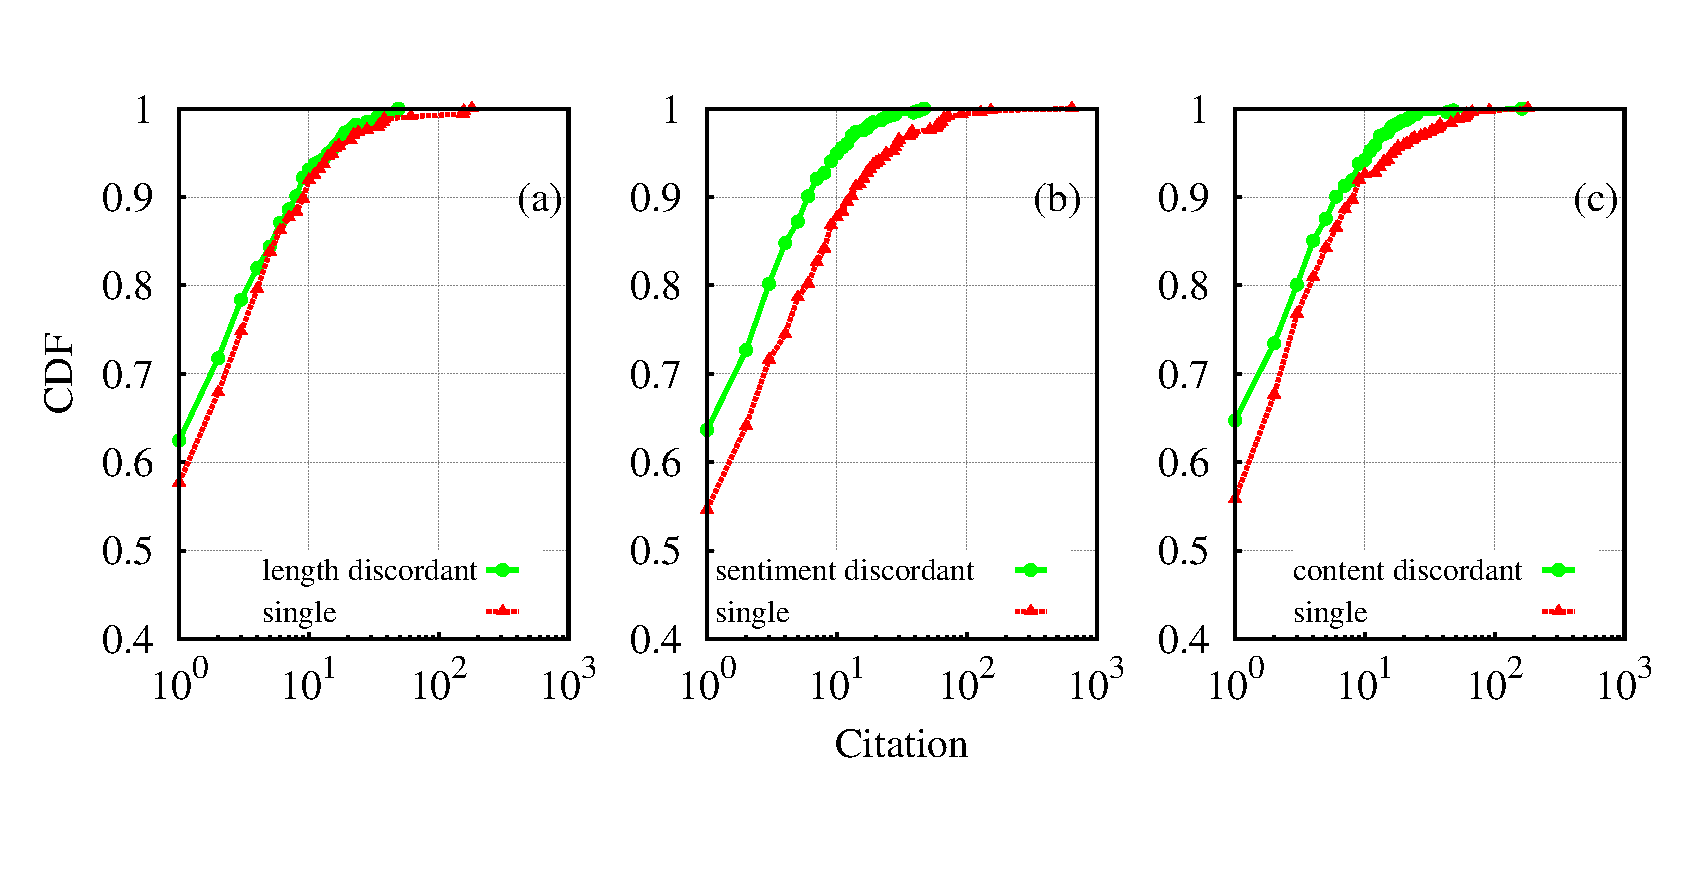
\includegraphics[scale = 0.3]{./texfiles/Chapter_4/cikm_17/figures/citation_mul_all_dis.eps}
 \caption{\label{con:citation_dis} Cumulative distribution function of citations for single refereed papers and discordant multi-refereed papers in terms of (a) length, (b) sentiment 
 and (c) content for JSTAT.} 
 %We randomly selected single-reviewed papers equal in number to the discordant multi-reviewed sets for each type.}
\end{figure}

\medskip
